\chapter{Evaluation} \label{chap:evaluation}

In this chapter we evaluate the work produced in this document. In \cref{sec:usability-theory} we evaluate the usability of the theory developed; in \cref{sec:usability-library} we assess the ease of use of the developed library; in \cref{sec:comparison-gillian} we compare the performance of the developed instantiations with their monolithic equivalent in Gillian; finally in \cref{sec:perf-pmap} we evaluate the performance improvement of the various \PMap{} optimisations.

\section{Theory Usability} \label{sec:usability-theory}

The theory we have presented contrasts with previous work for CSE engines in its use of resource algebras rather than partial commutative monoids or separation algebras. This allows us to easily prove the soundness of the presented constructions.

Still, some aspects of the theory can be at times somewhat unpractical to work with. Representing the empty memory $\bot$ as an element outside of an RA's carrier avoids common mistakes, but comes with the cost of requiring more ceremony when writing the rules for a state model transformers: in particular, we frequently need to define $\fn{wrap}$ and $\fn{unwrap}$ auxiliary functions to allow seamlessly handling the case where the state is $\bot$, which can clutter the rules. We note however that this additional care would also be needed with the PCM approach, though it would not be forced by the framework. The trade-off here is therefore between a more restrictive notation that avoids some errors, or a more flexible notation that can be error-prone.

The RA constructions presented are relatively primitive; in particular we only focus on simpler forms of ghost state, without exploring more advanced concepts that may make sense in a logic but not in an engine. The presented state models are sufficient to represent JavaScript, but fall short when attempting to model C, requiring specialised state models. For low-level languages where precision is required, it seems like one still needs to create a tailored state model, though transformers can still help alleviate the effort required. Other examples of this come to mind: for Gillian-Rust, the state model still needs to define the \statemodel{RustHeap}, \statemodel{Pcy} and \statemodel{Obs} state models \cite{gillianrust,sacha-phd}.\footnote{These state models have not yet been implemented in our library, though they exist as a monolithic construction as part of Gillian-Rust.} Though some of these are partly derived from other state models (\statemodel{RustHeap} uses \PMap), significant effort is needed to represent concepts such as prophecies or observations. It seems unavoidable for one to need to define some additional state models when targetting real-world languages. The fact these custom state models still use the generic constructions we defined show their versatility, and that they are still capable of simplfying part of the construction of a complex state model.

\section{Library Usability} \label{sec:usability-library}

The developed library exposes a total of 14 state models, including utility state models and optimised versions. These are all easy to use and combine when little additional functionality is required, for instance with WISL. Fine grained modifications of the constructions are also possible when needed, though sometimes non-trivial to implement. The effort needed to make an instantiation is much lesser than what would be required when creating the state model from scratch, as most behaviour is already available.

The key improvement our approach has over defining entire state models from scratch is \emph{verifiability}. Because all state models are relatively small (less than 400 lines) and isolated, ensuring a specific construction is sound is \emph{much easier} than verifying an entire state model is sound. Modifications to constructions are also relatively easy to verify, as they usually only impact a specific action or predicate, meaning one only needs to re-verify the soundness of the modified element. This is a major improvement on monolithic approaches, as verifying tightly coupled code spanning thousands of lines is no easy task.

\section{Comparison with Gillian Instantiations} \label{sec:comparison-gillian}

We now measure the performance of the instantiations created using our library against the performance of the original monolithic Gillian state models.

The evaluation is focused on testing the performance of state models across all modes supported by Gillian: whole program symbolic testing (WPST), OX verification and UX bi-abduction. The files tested are either small programs used to test the engine, or larger verification targets extracted from real world code. Furthermore, when possible, the tests are also run with different optimisations of $\PMap$: $\ALocPMap$ and $\SplitPMap$.

All test logs were verified to ensure full parity between all versions: the instantiations built using state model transformers yield the same results as the original instantiations. All passing tests pass, and all failing tests fail for the same reasons. All tests were run on a 2020 MacBook Pro, with an M1 processor and 8GB of memory.

This evaluation is split among the three different stacks originally supported by Gillian: WISL, JavaScript and C. A more in-depth presentation of the instantiations is done in \cref{sec:impl-instantiations}. We note that all Gillian instantiations make use of the abstract location optimisation internally, which as shown in \cref{sec:theory-optim-pmap} has some unsoundness issues. Therefore, to ensure our instantiations have the same results as the reference implementation, we evaluate our transformer constructions using the ALoc optimisation where relevant.

\subsection{WISL}

The WISL state model is $\PMap(\Loc, \Freeable(\List(\Ex(\Val))))$. The Gillian-WISL instantiation uses the abstract location optimisation, so our instantiations also do; using $\PMap$ without the optimisation would yield different test outcomes, due to its unsoundness. To measure the performance impact of different optimisations, we build the following transformer stacks: \begin{align}
\tag{TR}       & \ALocPMap(\Freeable(\List(\Ex(\Val)))) \\
\tag{TR-ALoc}  & \ALocPMap^\Str(\Freeable(\List(\Ex(\Val)))) \\
\tag{TR-Split} & \PMap_{\text{ALocSplit}}(\Freeable(\List(\Ex(\Val))))
\end{align}

Here $\PMap_{\text{ALocSplit}}$ represents a \PMap{} with both the ALoc and the split optimisations.

The benchmark is split into three parts: whole program symbolic testing (WPST), verification and bi-abduction, which are made up of respectively 1, 6 and 2 files. We note that the benchmark is small because it only has small code samples used for teaching purposes, rather than any real world code (since WISL is used for teaching). For this reason also we will not delve into too much detail for this comparison. The tests were run 50 times each, and the results are shown in \autoref{fig:wisl-perf-bars}.

\begin{figure}
\captionsetup{width=.4\linewidth}
\centering
\begin{minipage}[t]{.45\textwidth}
	\centering
	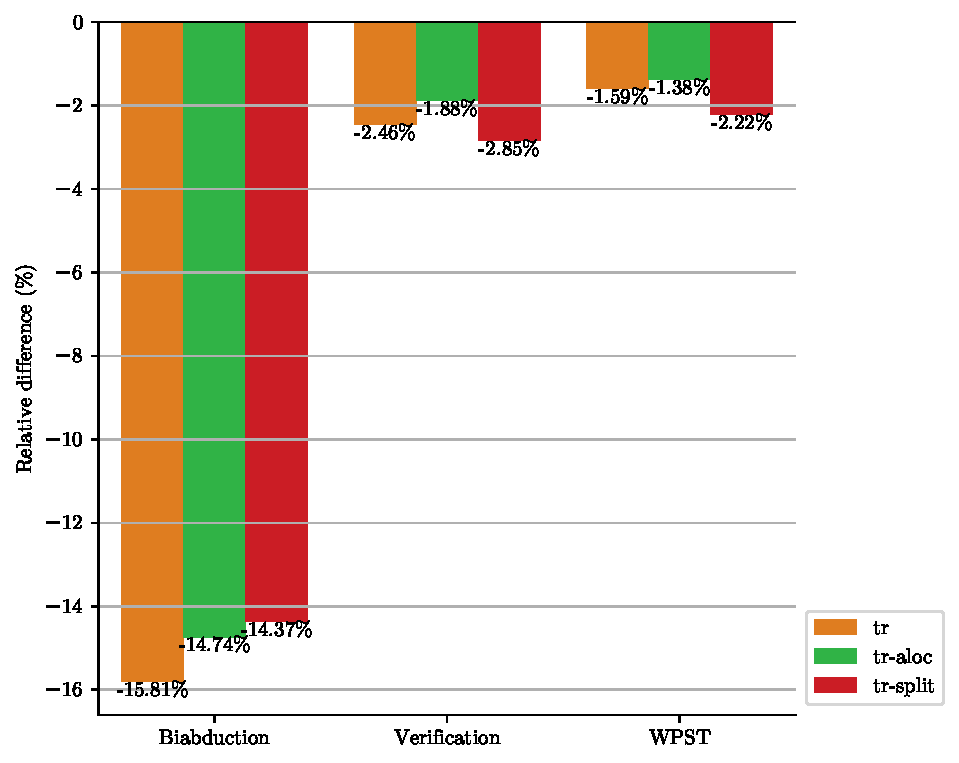
\includegraphics[width=7cm]{figures/wisl/avg_mode_relative_diff.pdf}
	\captionof{figure}{Average of the relative difference in execution time for different WISL test suites, per transformer stack}
	\label{fig:wisl-perf-bars}
\end{minipage}\hfill%
\begin{minipage}[t]{.45\textwidth}
	\centering
	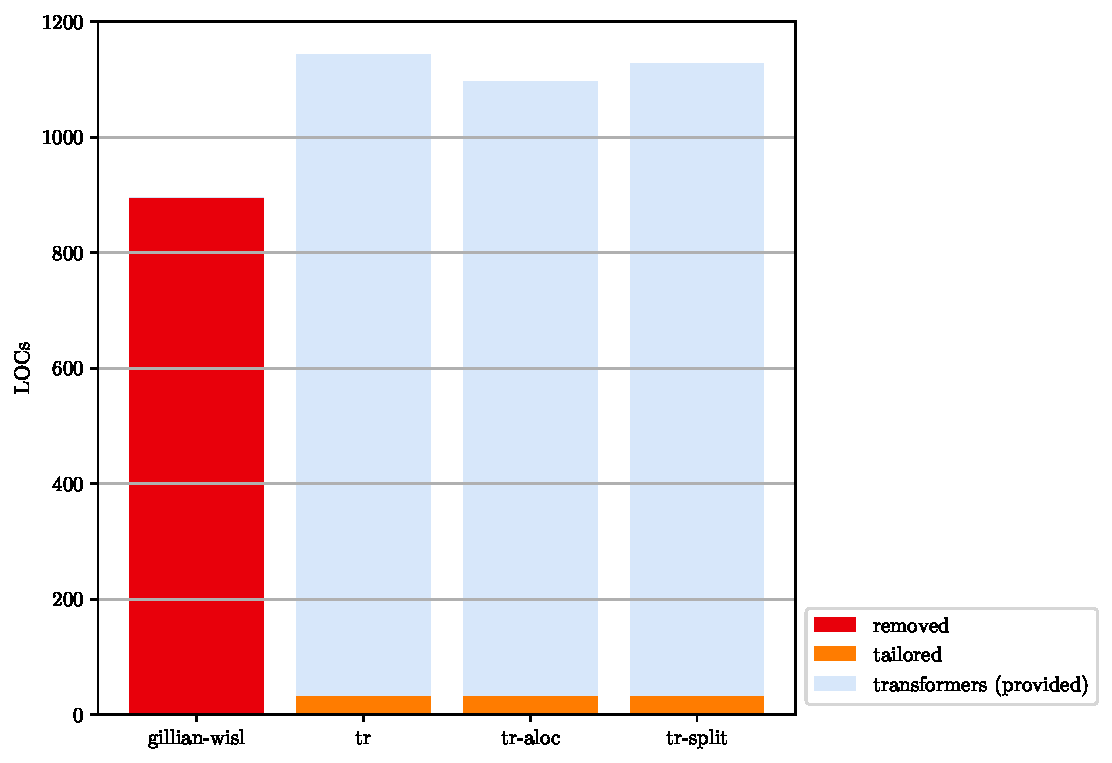
\includegraphics[width=7cm]{figures/wisl/locs.pdf}
	\captionof{figure}{Number of lines of code per WISL instantiation}
	\label{fig:wisl-locs}
\end{minipage}%
\end{figure}

The performance here seems to be worsened by the use of our library. This makes sense: WISL has a small toy-like state model, allowing for relatively simple code that can work straightforwardly. Gillian-WISL also uses an older and lower level API for Gillian, allowing it for instance to manipulate the PC without using \code{Delayed}. While this approach is more error-prone, it works well for small state models, and explains the better performance observed here. In comparison, using state model transformers is probably overkill and the added indirection worsens performance compared to a simple implementation. The difference is however negligible: no more than 3\% performance loss in verification and WPST.

While not a perfect measure of complexity, lines of code (LOCs) are used to compare the amount of code needed to instantiate each state model to get equivalent results. We only measure the lines of code in implementation files (\code{.ml}), ignoring interface files (\code{.mli}) and whitespace. What is gained from using transformers is a shorter implementation, as shown in \autoref{fig:wisl-locs}: the amount of work required from the developer has been reduced to almost none, as most functionality comes with the provided library. There are more LOCs needed as a whole, but the developer of the state model does not need to worry about the size of the library.

\subsection{JavaScript}

The JavaScript state model is $\PMap(\Loc, \DynPMap(\Str, \Ex(\Val)) \times \Ag(\Loc))$. Gillian-JS comes with some optimisations built-in, to improve performance. Firstly, it splits the first level $\PMap$ entries between concrete and symbolic \emph{values} (not keys!), avoiding substitutions in the concrete part. Secondly, it uses the abstract location mechanism described in \cref{sec:theory-optim-pmap}. Finally, it uses the OCaml \code{Hashtbl} module, a mutable data structure, rather than the immutable \code{Map} module; this avoids creating copies of the map on modification. All of these optimisations are important, as the state in JavaScript code tends to be significantly large, with the first $\PMap$ regularly reaching 200 to 600 entries when running real-world code: the highest recorded map size reaches 1179 entries for the \code{set3.gil} file.

To test all combinations of optimisations available via our library, we get the following four transformer stacks:
\begin{align}
\tag{TR}           & \ALocPMap(\DynPMap(\Str, \Ex(\Val)) \times \Ag(\Loc)) \\
\tag{TR-ALoc}      & \ALocPMap^\Str(\DynPMap(\Str, \Ex(\Val)) \times \Ag(\Loc)) \\
\tag{TR-Split}     & \ALocPMap(\SplitDynPMap(\Str, \Ex(\Val)) \times \Ag(\Loc)) \\
\tag{TR-ALocSplit} & \ALocPMap^\Str(\SplitDynPMap(\Str, \Ex(\Val)) \times \Ag(\Loc))
 \end{align}

The last version, TR-ALocSplit, is the closest in terms of applied optimisations to what Gillian-JS does. The biggest difference is the use of \code{Hashtbl}, as all transformers use immutable data structures.

Gillian-JS is capable of analysing real world code: the Buckets-JS\footnote{See \url{https://www.npmjs.com/package/buckets-js}.} library, which provides several data structures such as linked lists, dictionaries or sets has been verified by it, using whole program symbolic testing. Our instantiations having parity with the reference instantations, we are also capable of verifying Buckets-JS, with no additional modifications.

This benchmark is split into three parts: WPST, verification, and Buckets-JS (in WPST mode), which are made up of respectively 21, 6, and 78 files. All tests were then run 30 times, for each state transformer stack and for Gillian-JS (labelled ``base''). The results can be seen in \autoref{fig:js-perf-bars}. The first insight this give us is that transformers seem to, on the whole, outperform the monolithic Gillian-JS, with an improvement ranging from 2.8 to 6.9\%. We also see that the ALoc optimisation that uses strings as keys is the best improvement; the Split optimisation seems to have no effect, hinting that maybe the cost of splitting the map and checking what is concrete is too high to compensate the time gain on actual substitutions. We also note that the improvement given by the ALoc optimisation is greater when doing verification than with WPST; this is likely caused because verification uses more non-concrete locations, which implies less syntactic matches when doing lookups.

\begin{figure}
	\centering
	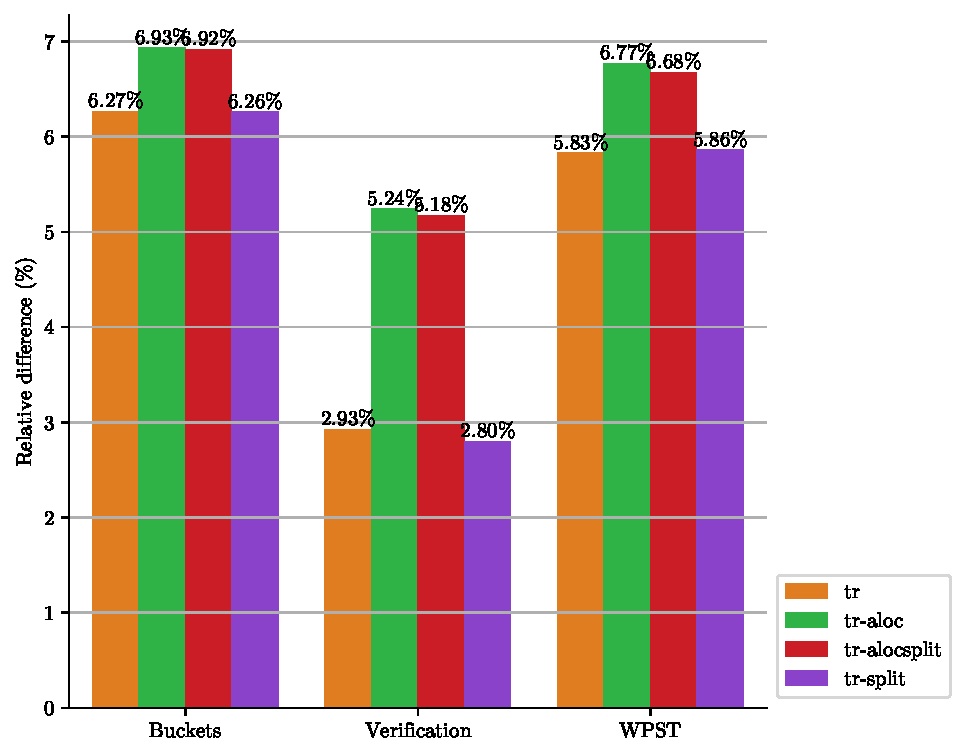
\includegraphics[width=8cm]{figures/js/avg_mode_relative_diff}
	\caption{Average of the relative difference in execution time for different JavaScript test suites, per transformer stack}
	\label{fig:js-perf-bars}
\end{figure}

The initial conclusion we can reach from this is that transformer stacks are more performant than the monolithic alternative. One could, of course, imagine that a hyper-optimised monolith could be made with optimisations specific to the state model, which would then out-perform the more generic transformers. However, in practice, the size of such monoliths makes these optimisations hard to apply, as code becomes complex quickly and makes changes harder. In contrast, transformers are very simple to optimise, as they maintain a more generic structure.

Another hypothesis this experiment seems to confirm is that the improvement given by optimisations is highly dependent on the context in which the engine is used: ALoc has a much lesser impact when doing WPST than when doing verification. Transformers thus allow users to tailor the optimisations they use in their stack according to what code is verified and how, by empirically measuring the performance of different alternatives (which are trivial to construct).

We may also take a closer look at how this time is spent within the engine. This is done by measuring the time before and after the entry point of each exposed method of the memory model and summing their difference. By looking at the average time per function call in the Buckets test suite (see \autoref{fig:js-avgtime-buckets}), we see that most memory actions (prefixed with ``ea/'', shorthand for \execac) are faster than in the base instantiation. Furthermore, copying is orders of magnitude faster with transformers, since no work needs to be done thanks to the use of immutable data structures.

\begin{figure}
	\centering
	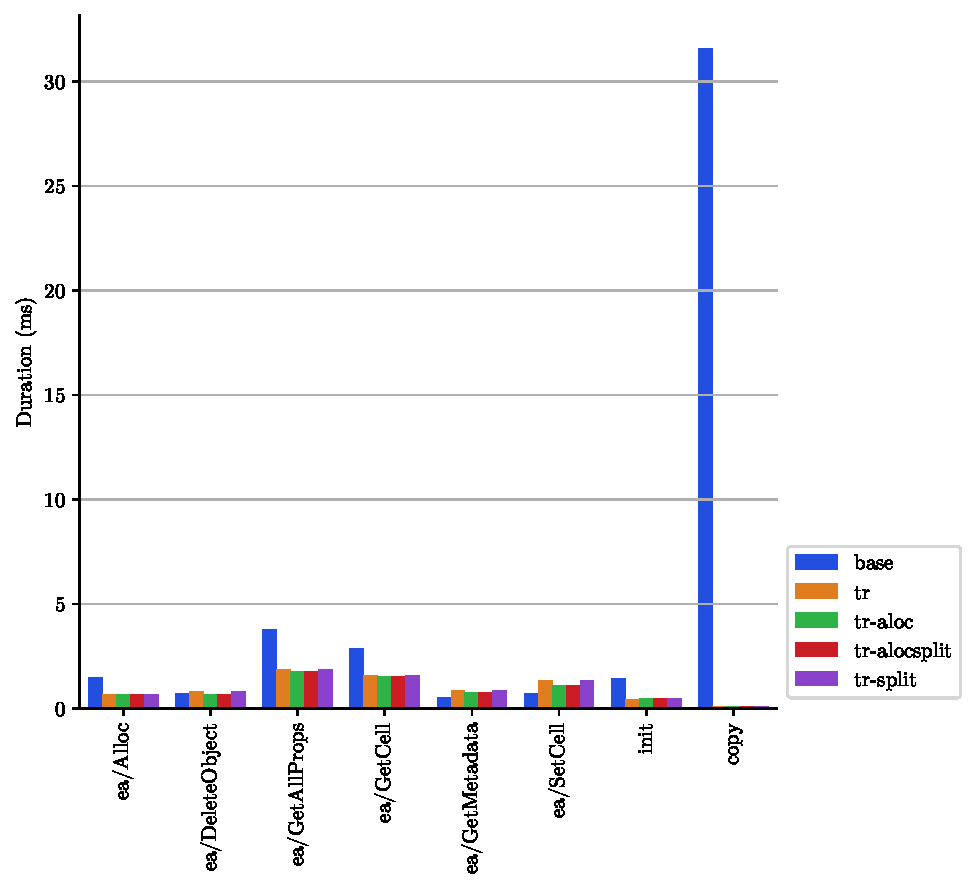
\includegraphics[width=8cm]{figures/js/buckets_avg_action_duration}
	\caption{Average time spent per 1000 function calls in the Buckets test suite}
	\label{fig:js-avgtime-buckets}
\end{figure}%

Looking at the average total duration for an execution of the test suite (see \autoref{fig:js-timespent-buckets}) however, we note that the time taken by copying the state is minimal, as seen by the size of the ``other'' category. Instead, most time is spent during the \load{} (\code{GetCell}) action, which is called 11400 times (more than twice as many times as \store{}). The most notable improvement from the transformer construction is the reduction of the time spent getting a cell, reducing total time spent by 43\% (from 28.55 to 16.18ms). Because \load{} dominates the amount of action calls (see \autoref{fig:js-callcount-buckets}), this is sufficient to make up for the performance loss in \store{} and ``\code{GetMetadata}'' (\load{} on the right side of the product).

\begin{figure}
\captionsetup{width=.4\linewidth}
\centering
\begin{minipage}[t]{.45\textwidth}
	\centering
	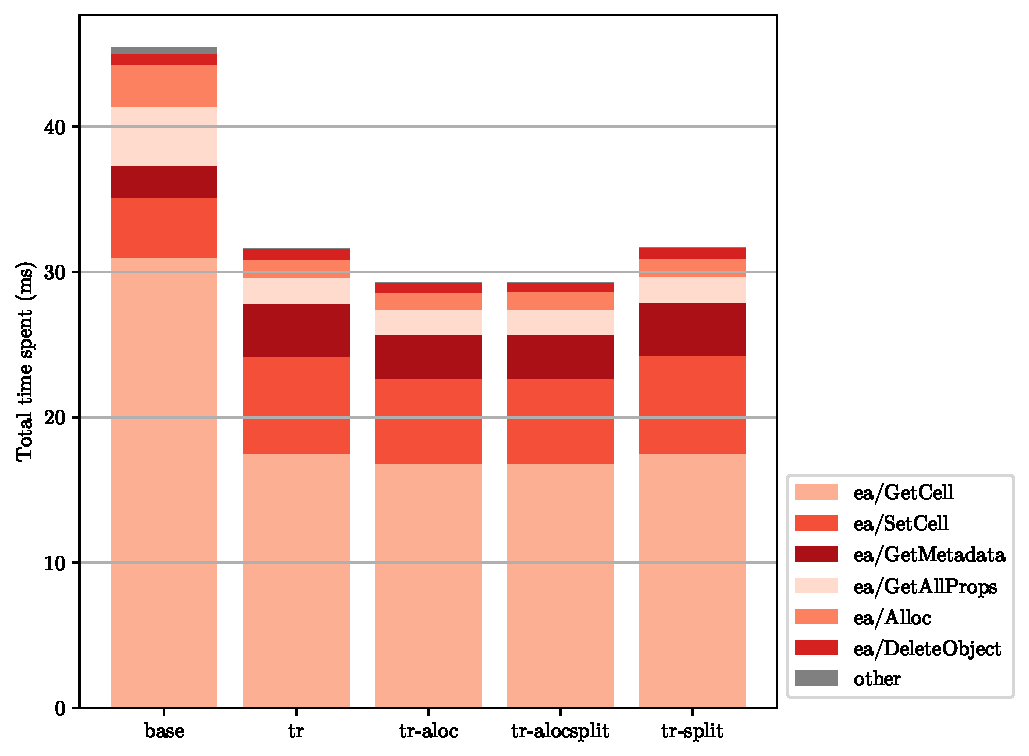
\includegraphics[width=7cm]{figures/js/buckets_time_spent_per_action_detailed.pdf}
	\captionof{figure}{Average total time spent per function in an execution of the Buckets test suite}
	\label{fig:js-timespent-buckets}
\end{minipage}\hfill%
\begin{minipage}[t]{.45\textwidth}
	\centering
	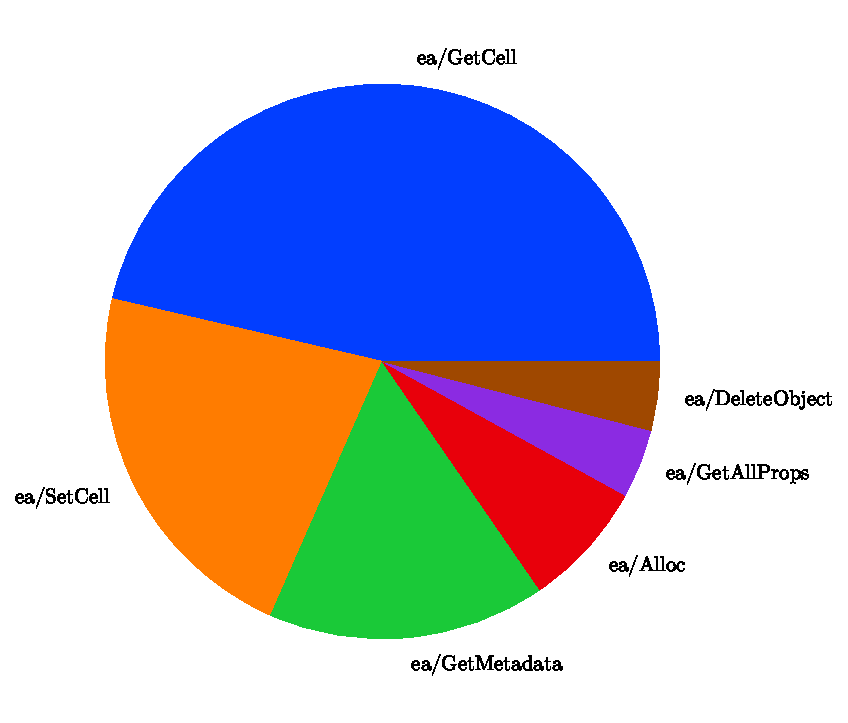
\includegraphics[width=7cm]{figures/js/buckets_avg_action_call_count.pdf}
	\captionof{figure}{Share of function calls for one execution of the Buckets test suite}
	\label{fig:js-callcount-buckets}
\end{minipage}%
\end{figure}

If, instead of focusing on WPST with the Buckets code we focus on verification, the picture painted is significantly different (see \autoref{fig:js-timespent-verif}). Indeed, while in WPST the memory model is only used for memory actions (as only the core engine is used), verification exercises the memory model quite differently, notably with \produce{} and \consume{}.

Most notably, this shows us that one of the leading differences in total time between different transformer instantiations is substitutions: TR and TR-Split spend more than twice as much time during substitutions than TR-ALoc and TR-ALocSplit. This is because with the ALoc optimisation, substitutions for the keys (abstract location names) can be filtered: if there is no substitution for abstract locations, we can simply map the values of the heap without worrying about key conflicts. Without this, substitutions need to be applied to both the key and the value, and then all resulting keys need to be compared to compose clashing entries -- this is expensive.

While this has not been measured, it is possible that the reason why Gillian-JS spends so little time in substitutions is because it uses mutable structures, allowing modifications to be done in-place, rather than creating new copies.

\begin{figure}
\captionsetup{width=.4\linewidth}
\centering
\begin{minipage}[t]{.45\textwidth}
	\centering
	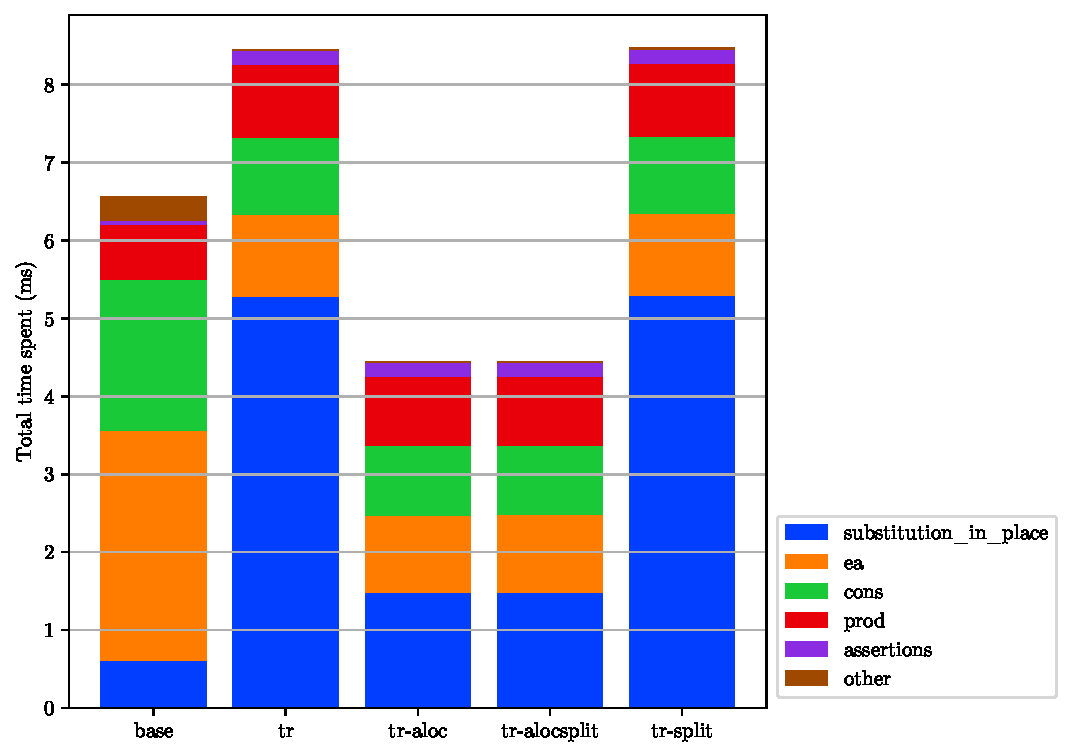
\includegraphics[width=7cm]{figures/js/verif_time_spent_per_action.pdf}
	\captionof{figure}{Share of grouped function calls for for one execution of the verification test suite}
	\label{fig:js-timespent-verif}
\end{minipage}\hfill%
\begin{minipage}[t]{.45\textwidth}
	\centering
	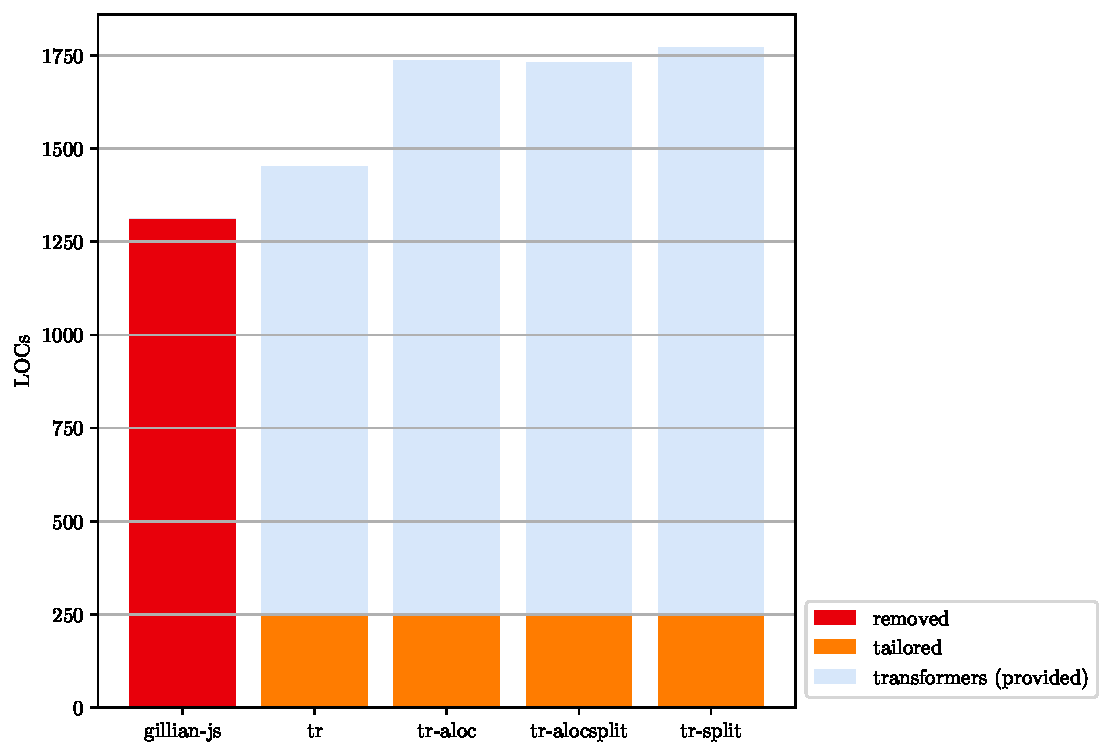
\includegraphics[width=7cm]{figures/js/locs.pdf}
	\captionof{figure}{Number of lines of code per JS instantiation}
	\label{fig:js-loc-count}
\end{minipage}%
\end{figure}

Substitutions aside, we note how significantly less time is spent in \execac{} and \consume{} calls compared to the base state model; about 65\% and 48\% respectively. Again, this seems to indicate that simpler transformers tend to be more efficient than large monoliths. We have not been able to pinpoint specific reasons for this. An hypothesis is that Gillian-JS overcomplicates its actions; for instance, the implementation of \code{GetCell} alone is over 100 lines long and is surprisingly intricate.

Finally, we may compare development effort between the two state models. The results are shown in \autoref{fig:js-loc-count}. Here, we note that the amount of tailored code needed for each instantiation (in yellow) is minimal compared to Gillian-JS: only 246 LOCs. Most of the LOCs are in the state model library, which is shared and can be reused for different state models; a user of the engine does not need to worry about them.

\subsection{C}

Gillian-C allows verifying a subset of the C language, via the CompCert-C verified compiler. Its state model can be defined as ${\PMap(\Loc,\Freeable(\BlockTree)) \times \CGEnv}$. To verify that the improvements from the optimised $\PMap$ versions are carried between instantiations, we also provide several C instantiations. Again we note Gillian-C already makes use of the ALoc optimisation, so in an effort to preserve parity we do not compare with instantiations that do not use it.
\begin{align}
\tag{TR}       & \ALocPMap(\Freeable(\BlockTree)) \times \CGEnv \\
\tag{TR-ALoc}  & \ALocPMap^\Str(\Freeable(\BlockTree)) \times \CGEnv \\
\tag{TR-Split} & \PMap_{\text{ALocSplit}}(\Freeable(\BlockTree)) \times \CGEnv
\end{align}

Like Gillian-JS, Gillian-C has been used to verify code that is used in real-world libraries. It verified the Collections-C library\footnote{See \url{https://github.com/srdja/Collections-C}.}, that provides data structures, using whole program symbolic testing, as well as the AWS encryption SDK\footnote{See \url{https://github.com/aws/aws-encryption-sdk-c}.}, an encryption library, using OX verification. Our instantiation is also capable of verifying these two libraries, providing the exact same results as the original Gillian instantiation.

This benchmark is split into five parts: WPST, verification, bi-abduction, \mbox{Collections-C} (in WPST mode) and AWS (in verification mode), each made up of respectively 8, 6, 7, 159, and 10 files. All tests were run 50 times, except the AWS test suite that was executed 10 times\footnote{This is because verifying the AWS code takes \emph{significantly} longer than the rest, due to its size.}.

The general results can be seen in \autoref{fig:c-perf-bars}. Here again, we note a significant performance improvement compared to the monolithic Gillian-C, in particular for the AWS and bi-abduction suites. As for the optimisations, we get inconsistent results: they seem to slightly improve performance for all modes but for AWS.

\begin{figure}
	\centering
	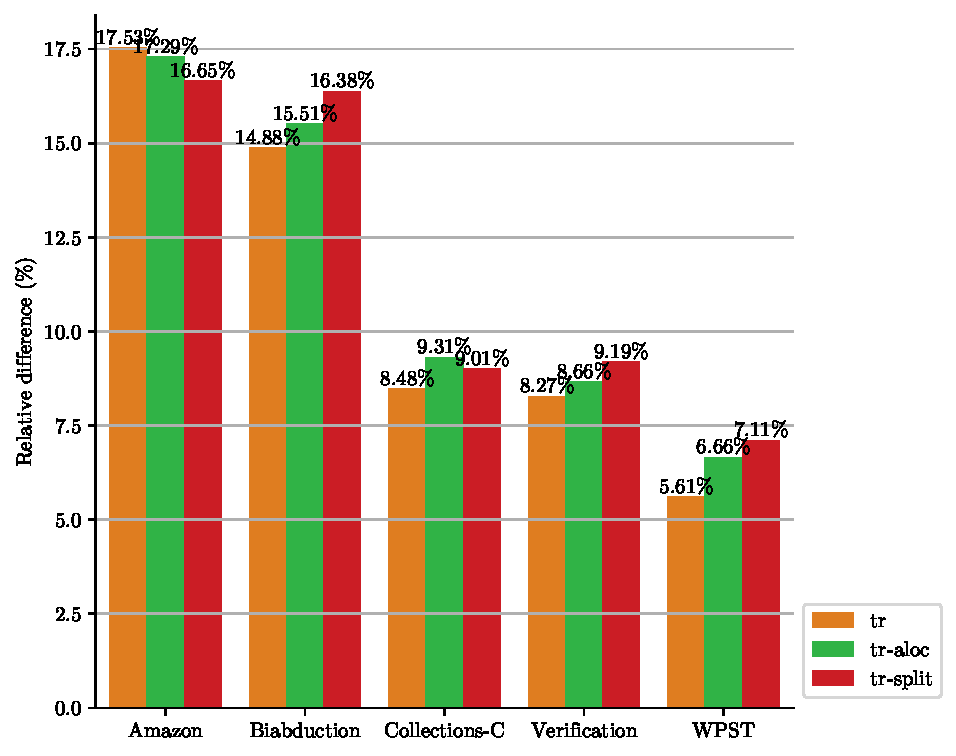
\includegraphics[width=8cm]{figures/c/avg_mode_relative_diff.pdf}
	\caption{Average of the relative difference in execution time for different C test suites, per transformer stack}
	\label{fig:c-perf-bars}
\end{figure}

We may now look into the detailed rundown of the time spent; we will focus on Collections-C WPST and the AWS encryption SDK verification, as these correspond to real-world code usage.

For Collections-C, when looking at the time spent in each function for each instantiation (see \autoref{fig:c-timespent-collectionsc}), the main takeaway is that the two most common actions, $\code{mem\_store}$ and $\code{mem\_load}$, are both faster than the original version; about 20\% and 25\% respectively. This is a crucial improvement, considering more than 75\% of memory actions in Collections-C is a load or a store.

The story is however wildly different for AWS code, which uses verification rather than WPST. Here, memory actions only represent a fraction of the total time spent, which is instead dominated by \consume, as seen in \autoref{fig:c-timespent-aws}. Here we note slight improvements in time for most categories, again seeming to indicate that the more generic approach is generally more performant, though the exact reason as to why is still unclear.

\begin{figure}
\centering
\begin{minipage}[t]{.45\textwidth}
	\centering
	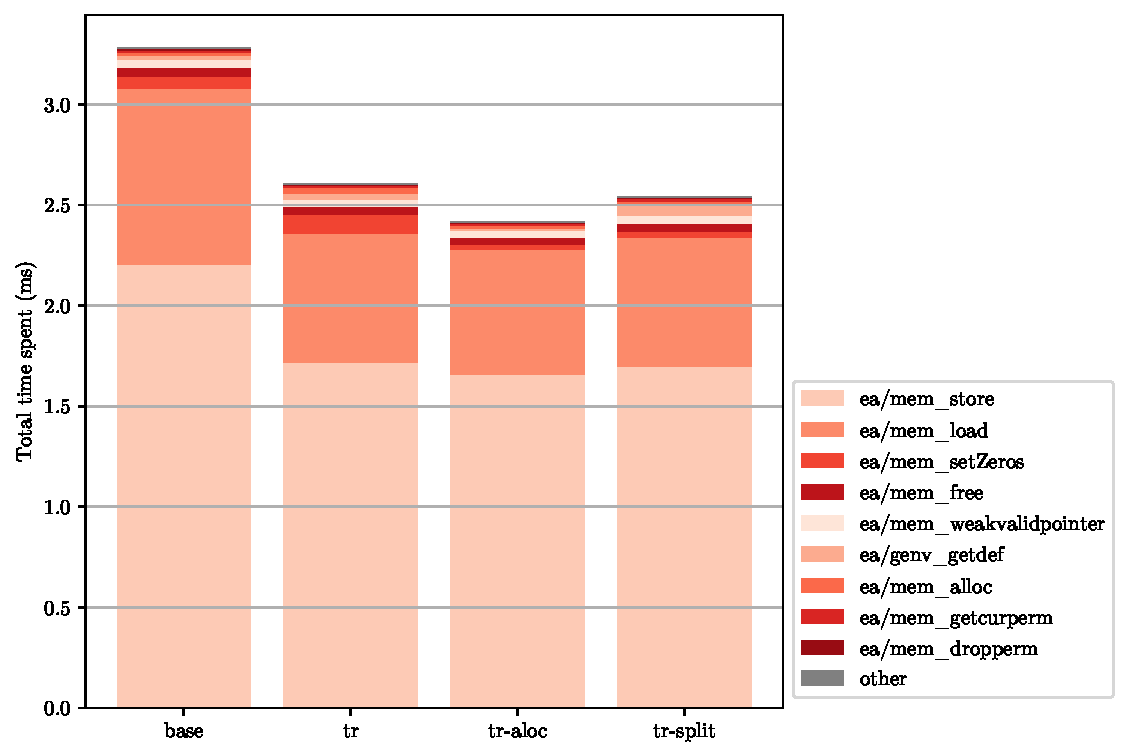
\includegraphics[width=7cm]{figures/c/collectionsc_time_spent_per_action_detailed.pdf}
	\captionof{figure}{Average total time spent per function in an execution of the Collections-C test suite}
	\label{fig:c-timespent-collectionsc}
\end{minipage}\hfill%
\begin{minipage}[t]{.45\textwidth}
	\centering
	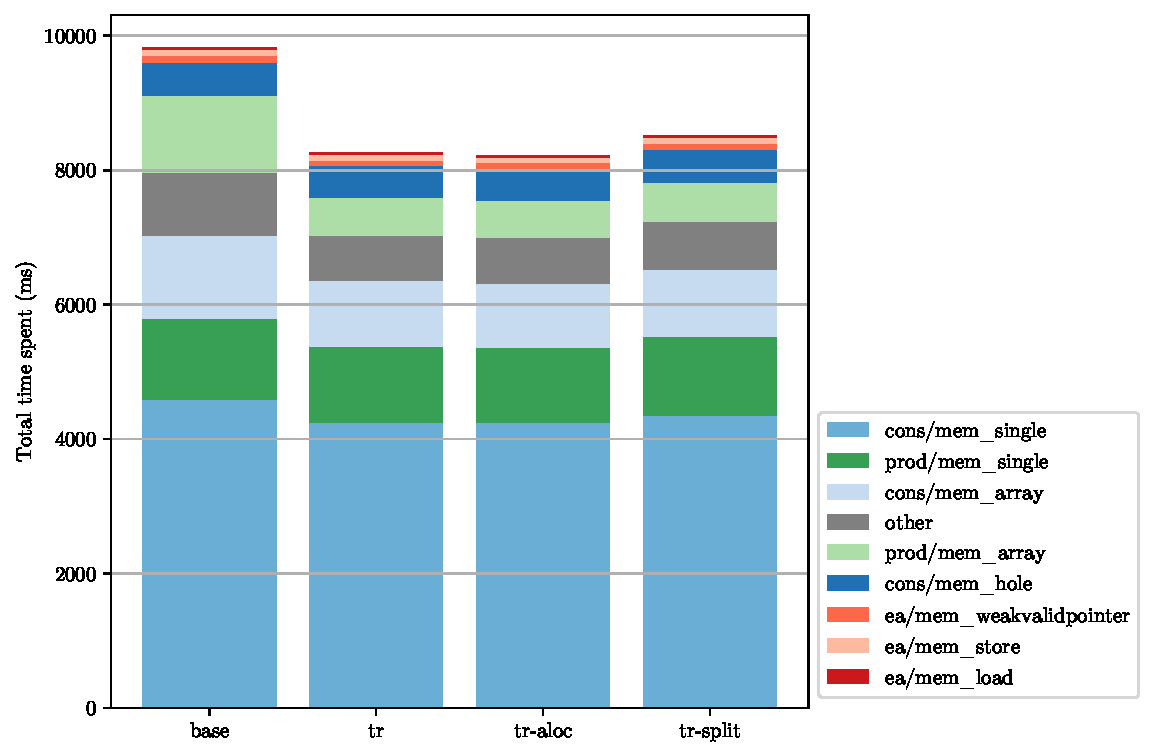
\includegraphics[width=7cm]{figures/c/aws_time_spent_per_action_detailed.pdf}
	\captionof{figure}{Average total time spent per function in an execution of the AWS header encryption SDK test suite}
	\label{fig:c-timespent-aws}
\end{minipage}%
\end{figure}

The charts for TR, TR-ALoc and TR-Split are extremely similar, for both Collections-C and AWS code; we can thus hardly make a hypothesis as to which optimisation is better suited. This is in part due to the fact these optimisations excel in larger maps, as was the case for JavaScript. In C, maps are instead rather small; for Collections-C, the map size tends to fluctuate between 15 and 35 elements, with the maximum recorder reaching 52 elements. For AWS, its size is between 10 and 20 elements, maxing at 20. This in particular explains why the optimisations are at times detrimental for the AWS test suite: because the maps are always small, the cost of both optimisations regularly outweighs their improvement.

We now compare the complexity of instantiations, using LOCs, delving into more details on the cause of each line count metric; see \autoref{fig:c-loc-count}. In particular, we see that the majority of the state model is the same; the modified part representing $\BlockTree$ and $\CGEnv$, which are lightly modified to fit into the transformers setup, while the untouched part represents the internal modules used by the C instantiations (for instance, to encode permissions, or memory chunks). Finally, the removed part of the code is trivially replaced with constructions, using $\PMap$ and $\Freeable$. Some tailored code is also required, to ensure the construction matches the interface of Gillian-C. This again shows that even for more complex state models that require a significant amount of custom code, using our state model library reduces the amount of code required exclusively for that instantiation, while providing performance gains for free.

\begin{figure}
	\centering
	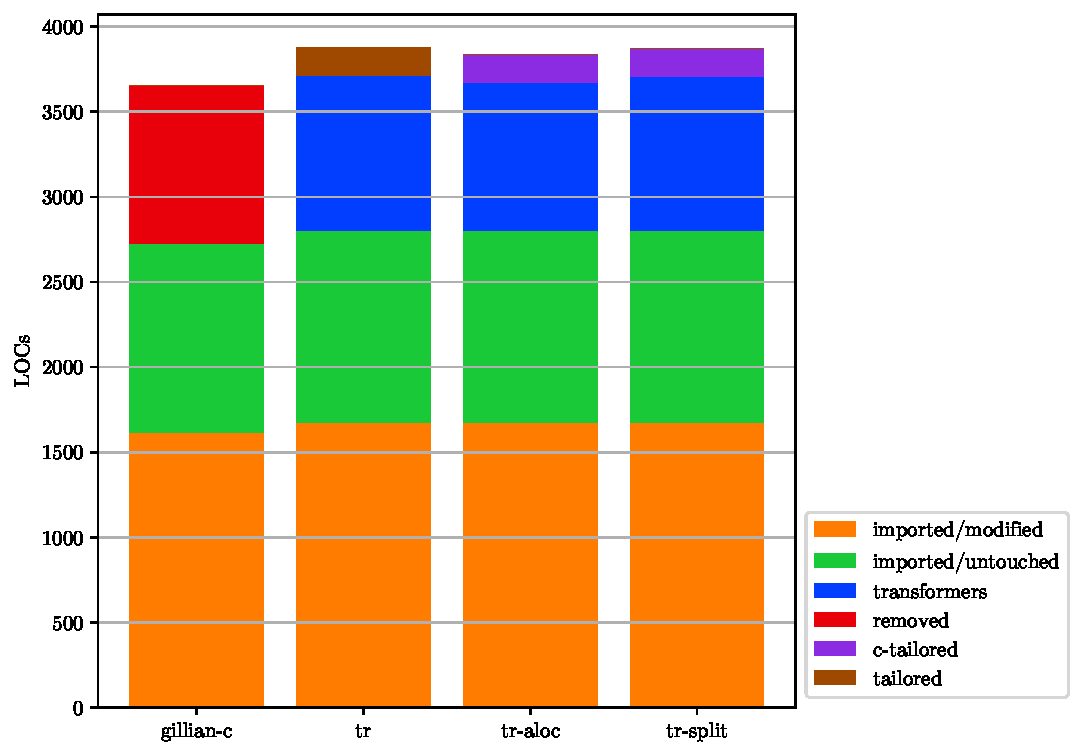
\includegraphics[width=7cm]{figures/c/locs.pdf}
	\caption{Number of lines of code per C instantiation}
	\label{fig:c-loc-count}
\end{figure}

\section{Partial Map Performance} \label{sec:perf-pmap}

Finally, and to confirm our intuition, we do a brief evaluation of the time taken to symbolically \code{get} elements from the different \PMap{} optimisations. This is done by measuring the time at the start and end of the \code{validate\_index} function of the various \PMap{} implementations during the execution of the Buckets-JS tests.\footnote{We choose to do it over this sample because it represents real-world code, and because JavaScript makes use of more combinations of optimisations, since the \PMap{} for objects does not have a \Loc{} domain.} The results are shown in \autoref{fig:pmap-perf}. \code{unopti} is the base \PMap{} implementation with no optimisation, \code{split} is \SplitPMap, \code{aloc} is \ALocPMap, and \code{aloc-str} is $\ALocPMap^\Str$ -- the ALoc optimisation with strings as keys.

\begin{figure}
	\centering
	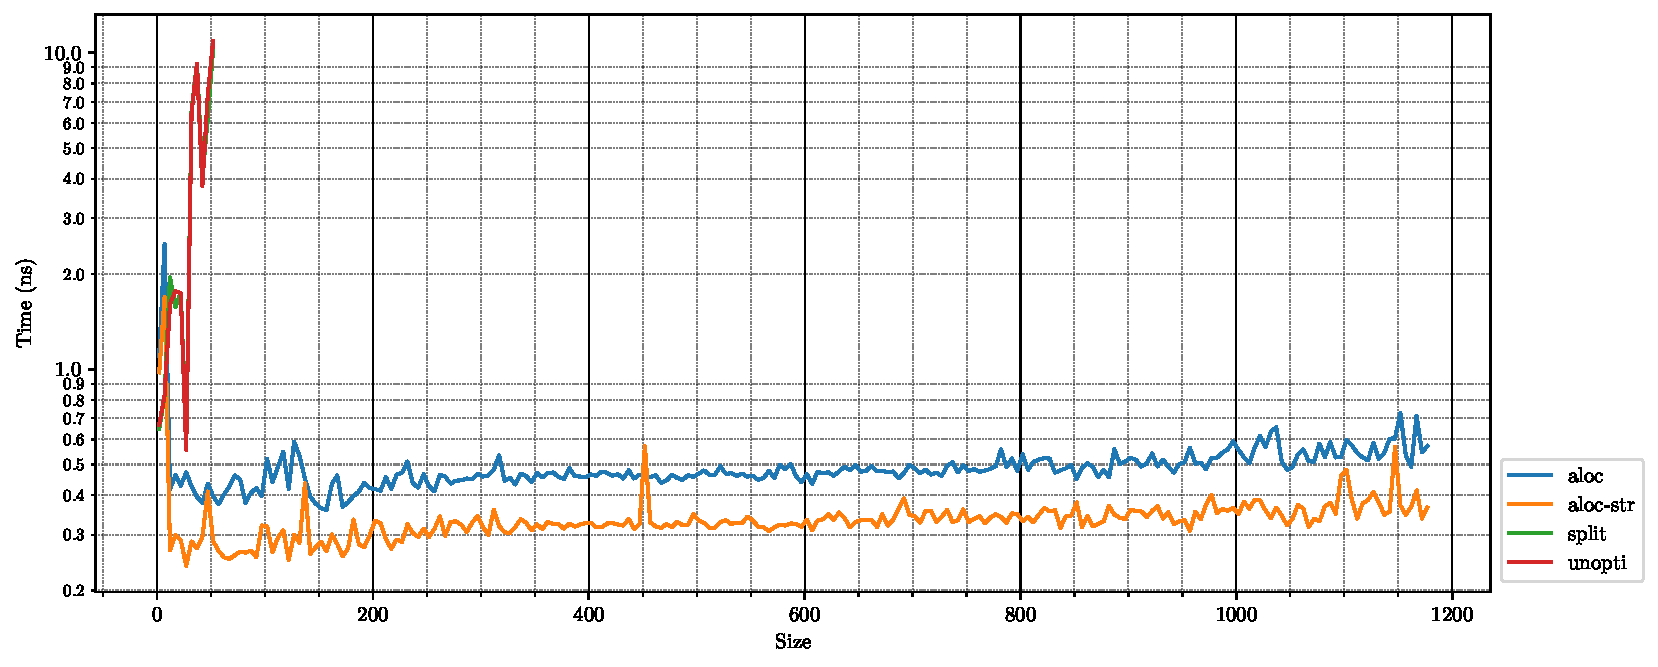
\includegraphics[width=13cm]{figures/pmap_time_per_size.pdf}
	\caption{Average time taken to access states in \PMap, depending on the size of the heap and the optimisations used.}
	\label{fig:pmap-perf}
\end{figure}

We first notice the significant difference between the \PMap{} with and without the ALoc optimisation: while the data only exists for map sizes up to 50 elements, the operation takes up to 10ns without ALocs, while taking on average 0.5ns with them. The use of the split optimisation does not seem to have an impact in this regard.

We can also compare performance when using expressions as keys (\code{aloc}) against using strings (\code{aloc-str}); here the impact seems to be constant, with an approximate improvement of 30\% when using strings. In both cases, the time taken for a lookup seems to logarithmically scale with the size, which makes sense given \code{Map}, the used data structure, is a balanced binary tree.
